\documentclass[11pt, english]{article}
        \usepackage{geometry}
                \geometry{
                        a4paper,total={210mm,297mm},
                        tmargin=32mm,
                        bmargin=32mm,
                        lmargin=26mm,
                        rmargin=26mm,
                }

	\usepackage{titlesec}
                \titleformat{\section}
                        {\normalfont\fontsize{18}{16}\bfseries}{\thesection}{0.5em}{}
                \titleformat{\subsection}
                        {\normalfont\fontsize{14}{16}\bfseries}{\thesubsection}{1em}{}
                \titleformat{\subsubsection}
                        {\normalfont\fontsize{11}{16}\bfseries}{\thesubsubsection}{1em}{}

	\usepackage{float}

	\usepackage{longtable}
        \usepackage{multirow}

	\usepackage{caption}
                \captionsetup[table]{labelfont=bf,textfont=bf,font=small,skip=8pt}
                \captionsetup[figure]{labelfont=bf,textfont=bf,font=small,skip=8pt}
        \usepackage{subcaption}
                \captionsetup[subtable]{labelfont=rm,textfont=rm,font=small,skip=8pt,labelformat=parens,labelsep=space}
                \captionsetup[subfigure]{labelfont=rm,textfont=rm,font=small,skip=8pt,labelformat=parens,labelsep=space}

	\renewcommand{\thetable}
                {\thesection.\arabic{table}}                                                         
	\renewcommand{\thesubtable}
                {\roman{subtable}}

	\renewcommand{\thefigure}
                {\thesection.\arabic{figure}}
        \renewcommand{\thesubfigure}
                {\roman{subfigure}}

        \usepackage{hyperref}
                \hypersetup{
                        colorlinks=true,
                        linkcolor=black,
                        filecolor=magenta,
                        urlcolor=cyan,
                        }

        \setlength{\parindent}{0pt}
        \renewcommand{\baselinestretch}{1.25}
        \usepackage{setspace}

        \usepackage{amsmath}
        \usepackage{amssymb}

	\usepackage{graphicx}

	\usepackage{tikz}
                \usetikzlibrary{trees,arrows,topaths}

	\usepackage[utf8]{inputenc}
	\usepackage[T1]{fontenc}

	\usepackage{lscape}
	\usepackage{colortbl}

\begin{document}

\pagenumbering{gobble}

	\title{\textsc{CS993 Software Engineering\\ Coursework Assignment}}
	\author{\href{http://lewisbritton.com}{\textsc{Lewis Britton}}}
	\date{\textsc{Academic Year 2021/2022}}
        \maketitle

\newpage

\pagenumbering{roman}

	\renewcommand{\contentsname}{Table of Contents}

	\tableofcontents

\newpage

\pagenumbering{arabic}

\section{Introduction \& Background}

	The system featured in this project is a functional GPS web application which is designed to provide users with detailed information, guidance and recommendations surrounding sport and leisure in the fine Scottish rural outdoors and Highlands. Or in other words, ``these mist covered mountains are home now for me, but my home is the lowlands and always will be''. That is, the application (which may also subsequently be referred to as `site') is focussed on guiding users through two primary activities (a `theme', if you will): hiking and cycling. Therefore, there is generally just one user type. Well, two if you include the one administrator; me. But all things admin are controlled internally so this doesn't count. However, these users may arrive at the site for many different reasons. Reasons which will become apparent as we look deeper into the functionality of the site.

	\subsection{Purpose}

	The purpose of this application is primarily to allow users to plan and record their progress and grow their abilities in the hills and on the road. Therefore, making GPS navigation through GPX analysis and location-based (including many more variables such as condition, weather, ability, etc.) route finding absolutely necessary. Essentailly, the purpose of this development is to encourage a \textit{burning} desire to compete with yourself and others from your very deepest \textit{roots}. Given this opportunity, users should view all of the finest details of their progress and be motivated to expand their scale and scope of opportunity and in effect, ability and passion. Hence, to quote from existing homepage:\\

	``Every passionate outdoorsman has that \textit{burning} desire for freedom in the sweet country air; to love what you do and to keep improving. Sometimes it takes effort from your deepest \textit{roots} to obtain PR after PR. So, with this fully interactive and informative GPS mapping application, take to the trails and the roads with more motivation than ever; being the fastest, most efficient, most prepared and the most endured athlete on your \textit{routes}. Burning Roots allows you to plan and optimize routes more precisely than ever before. Either create your routes manually or import existing ones from a GPX file to get started.''

	\subsection{Users}

	As discussed, users of this site will be sport/leisure oriented. Specifically, in the fields of hiking and cycling. Hiking is a vast umbrealla term which expands to everyone from hillwalkers through summer hikers, scramblers, climbers, free-soloers, mountaineers, all the way to ice climbers and extreme mountaineers. So the content, functionality and expansibility should all be in place to ensure they have a home to house their progress.\\

	On the other hand, the road cycling portion of the application focuses solely on road cyclists. Yes I may be biased, but that's because I'm an extremely keen road cyclist myself (and hiker, if you can't already tell). In fact, if I had the ability and time, this application would expand all the way throughout tennis and walking too. But unfortunately I'm not the Zuck'. Much like the hiking component, the cycling one is based on expanding scope of exploration, hence the road orientation as opposed to mountain biking etc. In an ideal world, as mountain biking is also considered an exploratory method in the context of hill ride-ins or trails, this application would include elements of it too. However, I simply don't know enough about it because I'm just a roadie. So forth, in a fully comprehensive environment, this application will house as many components of these sports as possible.

	\subsection{Development Process}

	As this is a solo project, there is no need for extensive use of inane project management methods such as team-based allocation or associated time or progress management.Therefore, there is no formal adherence to development frameworks such as agile. The initial structure of the site is the most important element when determining how the user will interact with the various aspects of their sport. Therefore, drafting the user interface (UI) is the most important step to understanding this. So forth, the development process of this system is as follows: requirement analysis $\rightarrow$ structural design $\rightarrow$ graphical user interface functionality $\rightarrow$ rear-end data management system functionality and connectivity $\rightarrow$ graphical user interface graphic design $\rightarrow$ testing. The application is basically a comprehensive data management system so, it will of course follow a beautiful 2007 format which is composed of the finset aspects of HTML, CSS. Depending on the requirement for users to better-access their data in the future and the available development time, there may be various aspects of PHP and SQL (using MySQL) implemented to manage this. JavaScript (JavaBloat) is also used to add `necessary' dynamics to the site and manage requests with JSON data files.\\

	For the easing of the writer's mental state, and the minimization of nugatory methodologies and bloated task flow donkeys such as IDEs or froymeworks, all elements are composed and performed by Lewis Britton in Bram Moolenaar's Neo Vi Improved. All write-up documentation is transcribed using Donald E. Knuth's \TeX. Or as some neomodernists like to use, \LaTeX. Due to time constraints, I will not be able to master the fine art of GNU Troff so, transcriptions may not be optimal without the Groff-PostScript combo.

\newpage

\section{Requirements}

	A clear base of requirements provide a blueprint upon which a project can be optimally developed with the user in mind. Understanding what the user specifically wants will help provide an idea of exactly how the software could/should collect information, store data, transact data and output data/information. In this case, conducting market research using existing services and applications which provide a similar result to this project is the best way to convey user-centered development. Therefore, cross comparison of applications such as Strava, Garmin Connect, Walkhighlands and Ordnance Survey provides a clear idea of what users already want and use but also, what there is room for in the market. As a very frequent user of all four of the discussed applications, I am also a useful tool to bring to light any possible extensions and enhancements on them which could be developed and implemented upon this system.

	\subsection{Scale \& Scope}

	As of the initialization stages of this project, there are a few points which are worth mentioning regarding the overall scalability of the project. That is, this system, if designed professionally, would be very large scale and offer much expansible functionality. The system would be open to a very large scale of users and would provide them with a great scale of abilities. More specifically, in an ideal world, users would be able to expand the scale of their use of this system to their own desire in terms of, initially, what sports they wish to participate in. As sports differ, relevant statistics, information, guidance, and accessibility, etc. differ, making it more time consuming for the development team. In this case, just myself. Furthermore, this ties-in to the scope of each individual sport. Ideally, users should have the ability to fully customize their experience and interact with many varying elements across each sport. However, again due to time and development constraints, much of this scope must be generalized or limited. Although this may be a large scale/scope disadvantage, it  does however, help keep the system clean and concise in many areas. For example, locations in which user may input to assign various aspects of their profile such as abilities, equipment etc. These can then be applied on a wider scope later within other aspects of the system. 

	\subsection{Functional \& Non-Functional}

	Understanding the difference between what must be implemented to make things work (functional requirements) and what must be implemented to make things relevant (non-functional requirements) is a critical step in creating the structure of the system as it helps distinguish between and also make associations between elements of both the design and construction stages of development. Keeping these requirements at the centre of development throughout the entire process allows the correct amendment of development or, of requirements themselves as more functionalities and their tangible implementation given constraints may either become closer or further to/from reach.\\

	It would be no use randomly assigning requirements to development. To help better address the required functionality of a system, requirements should be analysed using some form of hierarchical tool in order to create a clearer path for the development process. In this case I opted to use the Must-Have/Should-Have/Could-Have/Won't-Have (MoSCoW) methodology. This helps pinpoint exactly what is essential to make the system function as intended, and what could be implemented to make the system behave optimally / provide suitable interactions. This generally translates to functional requirements averaging at top-priority and non-functional requirements averaging nearer bottom-priority. Note that:

	\begin{itemize}
	\setlength\itemsep{0cm}
		\item \textit{Must-Have} implementations refer to aspects of the system which must be present in order to make it basically functional and behave as it is intended and as the user desires.
		\item \textit{Should-Have} implementations refer to features of the system which should be implemented in order to make the essential features of the system more accessible and useable to the masses. They may also exist to improve efficiency, but go unnoticed by the user. They may offer additional functionality which makes the system more unique (or something of the sort) and therefore, more `creative' and attractive to users.
		\item \textit{Could-Have} implementations refer to aspects which may become present or relevant during the development of the former two. They may add additional functionality or usability to existing aspects or simply add final touches to the system overall. They are sometimes more contemporary.
		\item \textit{Won't Have} non-implementations refer to aspects of the system which aren't necessarily impossible or are of a nature which the system `can't have' but, which will probably be omitted or postponed due to constraints such as time, man-power, technical ability, finance, etc.
	\end{itemize}

	As discussed, there is no formal client-base for this project and the creation of the system. Therefore, the following initial requirements have been developed by myself based on existing software and my own desires regarding alike systems. This list is not exhaustive and will no doubt be significantly altered and expanded as the process continues and each requirement is developed in further detail.

		\subsubsection{Functional}

	Users and the system \textit{must have} the ability to:

	\begin{itemize}
	\setlength\itemsep{0cm}
		\item Log-in using a username and password (no bloated authentication)
		\item View, edit and request deletion of their account details such as name, residence, gender, height, weight and profile picture
		\item View an overview of their statistics and recent activities
		\item View their personal inputs such as `abilities' and `equipment'
		\item View a weather breakdown using real weather data (OpenWeather API)
		\item View their `rewards'
		\item View their ongoing `challenges and competitions'
		\item Produce results based on user inputs such as their abilities, equipment, rewards and competitions
		\item Access the user's location (Geolocation API)
		\item View an OS map (OS API)
		\item Use and create results from the user's location (OS API, OpenWeather API)
		\item View and create GPS routes
		\item Upload GPX files
	\end{itemize}

	Users and the system \textit{should have} the ability to:

	\begin{itemize}
	\setlength\itemsep{0cm}
		\item Choose a `priority sport' which will be displayed with priority in their overview section
		\item View their current location (latitude/longitude or grid co-ordinates) as two numbers upon request
		\item Use their grid coordinates to quick-request a `random' route suggestion
		\item Display various grid location markers on an OS map
		\item Display various routes on an OS map
		\item Display various guides based upon elements of the system
	\end{itemize}

		\subsubsection{Non-Functional}

	To ensure a stable and trustworthy system, users and the system will:

	\begin{itemize}
	\setlength\itemsep{0cm}
		\item Offer an appropriate and relevant user interface 
		\item Contain the appropriate accessibility standards
		\item Be ensured that their data is secure and accessible only for the correct purposes
	\end{itemize}

		\subsubsection{User Story}

	Putting yourself in the hypothetical context of a user is a good method of understanding a process and how to apply your solution to it. The following scenario puts discussed requirements into a context which would be very likely while using this system. So forth (`[...]' denotes a process executed based on requirements):\\

	``As a user, I want to be able to [log-in to the system] and [change my `priority sport'] from hiking to cycling so I can [see] my insane last three cycles where I hit three consecutive sub-tow-hour forty-milers. I then want to [check the mountain weather] for Sg\`{u}rr nan Coireachan this weekend as I heard there's inversion potential, but I don't know much about clouds so I want to be able to [read and match relevant information] about the clouds to the forecast data. I then want to [view GPX files] of available routes on this hill. I also got a new pair of Scarpa Manta Tech GTX's the other day so I want to [add these to my `equipment cache'] to see if my recommendation rating changes regarding route difficulty/conditions.''

	\subsection{User Accessibility}

	As this system could be accessed and used by literally anyone with access to the internet, it is arguably `essential' that all users are welcomed by features which ensure any possible impairities they may hold are considered in the user-centered approach. Accessibility does not only refer to disability however, there are also aspects of this which are simply relevant to easy and concise navigation for example, to prevent user boredom and exit.\\

	To ensure the system is suitable for all of these scenarios, the user interface (whether accessing the site through a browser or a mobile device (scaled site)) is clear and concise. It primarily uses the readable and elegant Sans-Serif font Garamond, with suitable font-sizing and color. Hue, saturation and luminance are all appropriately assigned to create proper readability of and the correct contrast between elements. And, the universally respected font-family Font Awesome is used to display appropriate symbols etc. in element transitioning and readability. Ideally, this leads to more efficient universal understanding and transitioning. Like all requirements, these aspects can be tested and reviewed at a later date.

\newpage

\section{Project Management}

	The primary goal for this project is to deliver a functional web application system by august of this year. To allocate the appropriate time and resources, this task can be broken down into smaller, more manageable sections to be executed along the way. The process of managing this involves time management, resource management, an understanding of the system layers, and an understanding of the tools used to manage the system's layers.

	\subsection{Life-Cycle}

	As discussed, no formal framework is followed during the life-cycle of the software development in this project. However, the project is divided into three intuitive sections which segment project planning; user interface functionality development, design and transactions; back-end data storage and transactions; and, testing processes. As each stage of the system development (front-end and back-end) involve intermediate testing, it could be argued that the life-cycle does follow the `sprint' concept of `Agile' in that project stages are assigned periods which involve constant reference to the user-centered approach of requirements and testing. Each stage of development also takes into account prioritization of requirements indicated by the MoSCoW hierarchy.\\
	
	Although, as always, I will simply be sticking to my Calcurse calendar client to indicate target dates and a plain text notes file to keep track of my progress and to-do tasks, a visual representation is often a `helpful' instrument in illustrating the project elements across both characterizations and time. This allows key milestones to be identified and tolerances to be allocated to each element. The following Gantt chart illustrates the major aspects of the development process. Note that a chart such as this is always subject to amendment and improvement as time goes on. It is used in the initial stages simply to provide a manageable overview. For simplicity, the chart runs from the first full week in May (w/c 2nd) until the final full week in July (w/e 31) (13 weeks).

	\vspace{\fill}

	\begin{center}
		\textsc{Turn \& Rotate Page}
	\end{center}

\newpage

\begin{landscape}

	\begin{table}[h]
		\tiny
		\renewcommand{\arraystretch}{1.25}
	\begin{center}
	\begin{tabular}{lll|cccccccccccccc}
		\textsc{\#} & \textsc{Task} & \textsc{Tools} & \textsc{W1} & \textsc{W2} & \textsc{W3} & \textsc{W4} & \textsc{W5} & \textsc{W6} & \textsc{W7} & \textsc{W8} & \textsc{W9} & \textsc{W10} & \textsc{W11} & \textsc{W12} & \textsc{W13}\\
		\hline
		\textbf{1.} & \textbf{Project Planning} &\\
		1.1. & Requirements Gathering & Brain & \cellcolor[gray]{0.1}\\ 
		1.2. & Requirements Implementation Planning & Brain & \cellcolor[gray]{0.1}\\
		1.3. & User Interface Structure & Brain & \cellcolor[gray]{0.1}\\
		1.4. & Rear-End Structure & Brain & \cellcolor[gray]{0.1}\\
		1.5. & Requirements Review & Brain & & \cellcolor[gray]{0.1}\\
		\hline
		\textbf{2.} & \textbf{User Interface (Front-End)} &\\
		2.1. & Functionality & HTML & & \cellcolor[gray]{0.1} & \cellcolor[gray]{0.1} & \cellcolor[gray]{0.1} & \cellcolor[gray]{0.1} & \cellcolor[gray]{0.1} & \cellcolor[gray]{0.1}\\
		2.2. & Communications \& Transactions & HTML, JavaScript & & \cellcolor[gray]{0.1} & \cellcolor[gray]{0.1} & \cellcolor[gray]{0.1} & \cellcolor[gray]{0.1} & \cellcolor[gray]{0.1} & \cellcolor[gray]{0.1}\\
		2.3. & Small Data Store & JavaScript, JSON & & \cellcolor[gray]{0.1} & \cellcolor[gray]{0.1} & \cellcolor[gray]{0.1} & \cellcolor[gray]{0.1} & \cellcolor[gray]{0.1} & \cellcolor[gray]{0.1}\\
		2.4. & Design \& Accessibility & CSS, JavaScript & & \cellcolor[gray]{0.1} & \cellcolor[gray]{0.1} & \cellcolor[gray]{0.1} & \cellcolor[gray]{0.1} & \cellcolor[gray]{0.1} & \cellcolor[gray]{0.1}\\
		2.5. & Element Testing & HTML, CSS, JavaScript & & & & & & \cellcolor[gray]{0.1} & \cellcolor[gray]{0.1}\\
		2.6. & Requirements Review & Brain & & & & & & & \cellcolor[gray]{0.1}\\
		\hline
		\textbf{3.} & \textbf{Data Store (Back-End)} &\\
		3.1. & Log-In Management & PHP/MySQL & & & & & & & & \cellcolor[gray]{0.1} & \cellcolor[gray]{0.1} & \cellcolor[gray]{0.1} & \cellcolor[gray]{0.1}\\
		3.2. & Large Data Store & PHP/MySQL & & & & & & & & \cellcolor[gray]{0.1} & \cellcolor[gray]{0.1} & \cellcolor[gray]{0.1} & \cellcolor[gray]{0.1}\\
		3.3. & Element Testing & HTML, PHP/MySQL & & & & & & & & & & \cellcolor[gray]{0.1} & \cellcolor[gray]{0.1} & \cellcolor[gray]{0.1}\\
		3.4. & Requirements Review & Brain & & & & & & & & & & & & \cellcolor[gray]{0.1}\\
		\hline
		\textbf{4.} & \textbf{Review \& Additional Testing}\\
		4.1. & Distribute System for Testing & E-Mail Server/Client, People & & & & & & & & & & & & \cellcolor[gray]{0.1} & \cellcolor[gray]{0.1}\\
		4.2. & Review Feedback \& Implement Changes & Various & & & & & & & & & & & & \cellcolor[gray]{0.1} & \cellcolor[gray]{0.1}\\
		4.3. & Repeat Process Until Satisfied & Various & & & & & & & & & & & & \cellcolor[gray]{0.1} & \cellcolor[gray]{0.1}\\
		\hline
	\end{tabular}
		\caption{Gantt Chart}
	\end{center}
	\end{table}

\end{landscape}

\newpage

	\subsection{Tools}

	As previously discussed, I will not be touching any bloated IDEs or other development environments throughout this process. All of my code is/will-be written in plain text, in the command line of course (running Suckless' DWM on Artix Linux), using Bram Moolenaar's NeoVim. This is what works for me; it's efficient, minimal and simply allows you to get your work done and done right. Therefore, all code created and provided is raw, with the following file extensions: .html, .css, .js, .php, .sql, .json, .csv. Supporting documentation in composed and transcribed using Donald E. Knuth's \LaTeX\ and compiled using pdflatex, resulting in the following file formats: .tex, .pdf. Other materials are provided in .txt and .md (Markdown) format.\\

	As a fan of Git and version control systems, I opted to use GitHub throughout this project to host all of my development content and documentation. Using a tool such as this provides assurance that your work is stored in a fairly `safe' place and insurance if anything goes wrong locally to your machine. For example, using Git Rollback/Revert to undo/alter changes or, simply restoring a backup in the event of data loss. As this system is a web application, the directories present within the relevant GitHub repository take the form of the tree of the final product. That is, the file/page path of the site. Therefore, all source code (HTML, CSS, JavaScript, PHP), supporting files (PHP, SQL, JSON, CSV) and documentation (TeX, PDF, TXT) is present, alongside a ReadMe (Markdown (MD)) file indicating the purpose and intended use of the system.

\newpage

\section{Design}

	This system works just like most others. It uses an attractive front end which allows users to view data and make requests to and from a semi-back-end and back-end. It allows these users to communicate with various computations and algorithms through inputs which translate to different pulls and manipulations of data on the back-end. Of course, this process adheres closely to the analysis of user requirements and functionality.\\

	After the consideration of the tangibility and feasibility of requirements and their relevance, understanding how to allow user to most easily interact with different elements is a crucial component to the project. Therefore, it is not practical to immediately start developing a data-oriented back end. Starting by laying-out elements in a logical order provides an initially useful idea of what the data flow will look like. This stage therefore involves fast prototyping and rapid changing and testing of elements. Understanding the structure of this stage gains you a perspective of the scope of the functionality of the system and the scalability given the time, technical and financial constraints.

	\subsection{User Interface Logical Design}

	This is a fairly comprehensive system, which naturally means it is open to use by all age groups, personalities, genders, races, etc., who care about fitness, the outdoors, or simply wish to try the features of the system. This means that the system must ideally be available on multiple platforms. These platforms must satisfy two major criteria: [1] they must be appropriate for all possible users (i.e. be available on any device of the user's choosing), and [2] they must be appropriate for the implied conditions in which the system will be used (i.e. a user may wish to use the OS GPS feature on their telephone while on a conquest).\\

	Hence, the decision to make this system a web application. Being a web application means this system can exist for purely functional reasons with and optional additional degree of `bloat' (i.e. the user interface) which makes the system (perceived as) more `attractive' by users. As a functional man, I'd ideally have this site looking like Harvard.edu in 2007 but sadly that just isn't what normies want this day so there'll be a little bit of `arty' CSS to satisfy those users who are a bit `extra'. This will be touched on more in the graphic design section. Anyway, all of this essentially means that the system is designed to be primarily used on a desktop machine (i.e. for the conquest planning features) and be fully scalable to mobile devices for use on mobile browsers, where it will visually take the form of a `mobile application' (i.e. for intra-conquest use such as the GPS features). Given a full development team, time and financial input, this system could be extended to a full mobile application in  which the GPS features can be used offline as many users will find themselves without an internet connection when in the field. This is primarily why the system is oriented more so towards the `planning' portion of conquests and not the `in-the-field' portion. The latter relies to much on the physical safety of the users and the scale and scope of this system simply cannot provide that given its constraints.\\

	So forth, in the preliminary stages of this project, the system is segmented into the relevant portions highlighted in the diagram below. This in no way resembles the structure of the final system however, does provide somewhat of an overview of how the user will navigate through the system. Note that as this system is not necessarily `object oriented' and is simply just supported by JavaScript objects in numerous areas, an object oriented diagram is not the most appropriate method of displaying the interface. I have opted for a recursion tree. In summary, a user logs-in, lands on their home page where they find their profile and attributes; and have the option to navigate to other pages which contain mapping and GPS abilities relevant to hiking and cycling. See below:

	\vspace{\fill}

	\begin{center}
		\textsc{Turn \& Rotate Page}
	\end{center}

\newpage

	\begin{landscape}

	\begin{center}

	\tikzstyle{level 1}=[level distance=1.5cm, sibling distance=8cm]
        \tikzstyle{level 2}=[level distance=2cm, sibling distance=2cm]
        \tikzstyle{level 3}=[level distance=3cm, sibling distance=1cm]

        \tikzstyle{bag} = [text width=7.5em, text centered]
        \tikzstyle{end} = [text width=9em, text centered]

        {\scriptsize\begin{tikzpicture}
                \node[bag] {Log-In}
                        child {
				node[bag] {Drafting Room (Landing)}
                                        child {
                                                node[end] {Site Intro/\\Summary}
                                                }
                                        child {
                                                node[end] {Profile\\Summary}
                                                        child {
								node[end] {Personal Details,\\Profile Picture}
                                                        }
                                                }
                                        child {
                                                node[end] {Profile\\Attributes}
                                                        child {
								node[end] {Overview (Stats to-Date,\\Recent Projects),\\Conditioning (Ability,\\Equipment,\\Weather),\\Rewards,\\Competitions}
                                                        }
                                                }
                                }
			child {
                                node[bag] {Hiking}
                                        child {
                                                node[end] {`Conquest'\\GPS Map}
                                                }
                                        child {
                                                node[end] {`Ranger'\\Status\\Graphs}
                                                }
                                        child {
                                                node[end] {GPS Routes}
                                                }
                                        child {
                                                node[end] {Key}
                                                }
                                }
                        child {
                                node[bag] {Cycling}
                                        child {
                                                node[end] {`Cruiser'\\GPS Map}
                                                }
                                        child {
                                                node[end] {`Ranger'\\Status\\Graphs}
                                                }
                                        child {
                                                node[end] {GPS Routes}
                                                }
                                        child {
                                                node[end] {Key}
                                                }
                                };
        \end{tikzpicture}}

	\end{center}

	\end{landscape}

\newpage

	\subsection{User Interface Graphic Design}

	A system's graphic design is often overlooked, especially in smaller, more functional developments such as this where there is lacking knowledge or specialization of the required artistic / graphic design skill and practices. This is why the styling portion of many applications in development is often outsources to commercial graphic design teams. This obviously is not the case in this scenario; all graphic design is developed using internal aspects of CSS, and desktop publishing and markup programs such as GIMP and Serif Page Plus for additional graphical content.\\

	In this context of `the outdoors' in a traditional setting, graphic design is not as relevant as it may be in other, more neomodernist-based, applications however, appropriate graphic design here can help distinguish between elements such as those relevant to hiking and cycling. For example, using color schemes, shape, texture, balance, etc., to represent aspects of the landscapes, activities and communities.

\newpage

	\subsection{Basic Prototype}

	Below is a basic prototype of some of the introductory features of this system. To-date, focus has been centered on gaining a solid idea of the overall structure of the system and implementing functionality of the three primary APIs used: Geolocation, OpenWeather and Ordnance Survey. As of this date, the OpenWeather API is fully functional, with Geolocation integration; the OS API is semi-functional, being viewable but not yet containing any interactive features. Note that the conditioning element of the profile section is the only one with existing content (apart from the separate OS map page), hence no view of the other profile elements.

	\begin{table}[h]
		\scriptsize
		\renewcommand{\arraystretch}{1.25}
	\begin{center}
	\begin{tabular}{ccc}
		Drafting Room (Landing) & Profile & Profile: Conditioning\\
		\includegraphics[width=4.25cm,height=7.5cm]{1.png} & \includegraphics[width=4.25cm,height=7.5cm]{2.png} & \includegraphics[width=4.25cm,height=7.5cm]{3.png}\\
		Profile: Conditioning $\rightarrow$ Weather & Navigation Drop-Down & Hiking: `Conquest' [OS] Map\\
		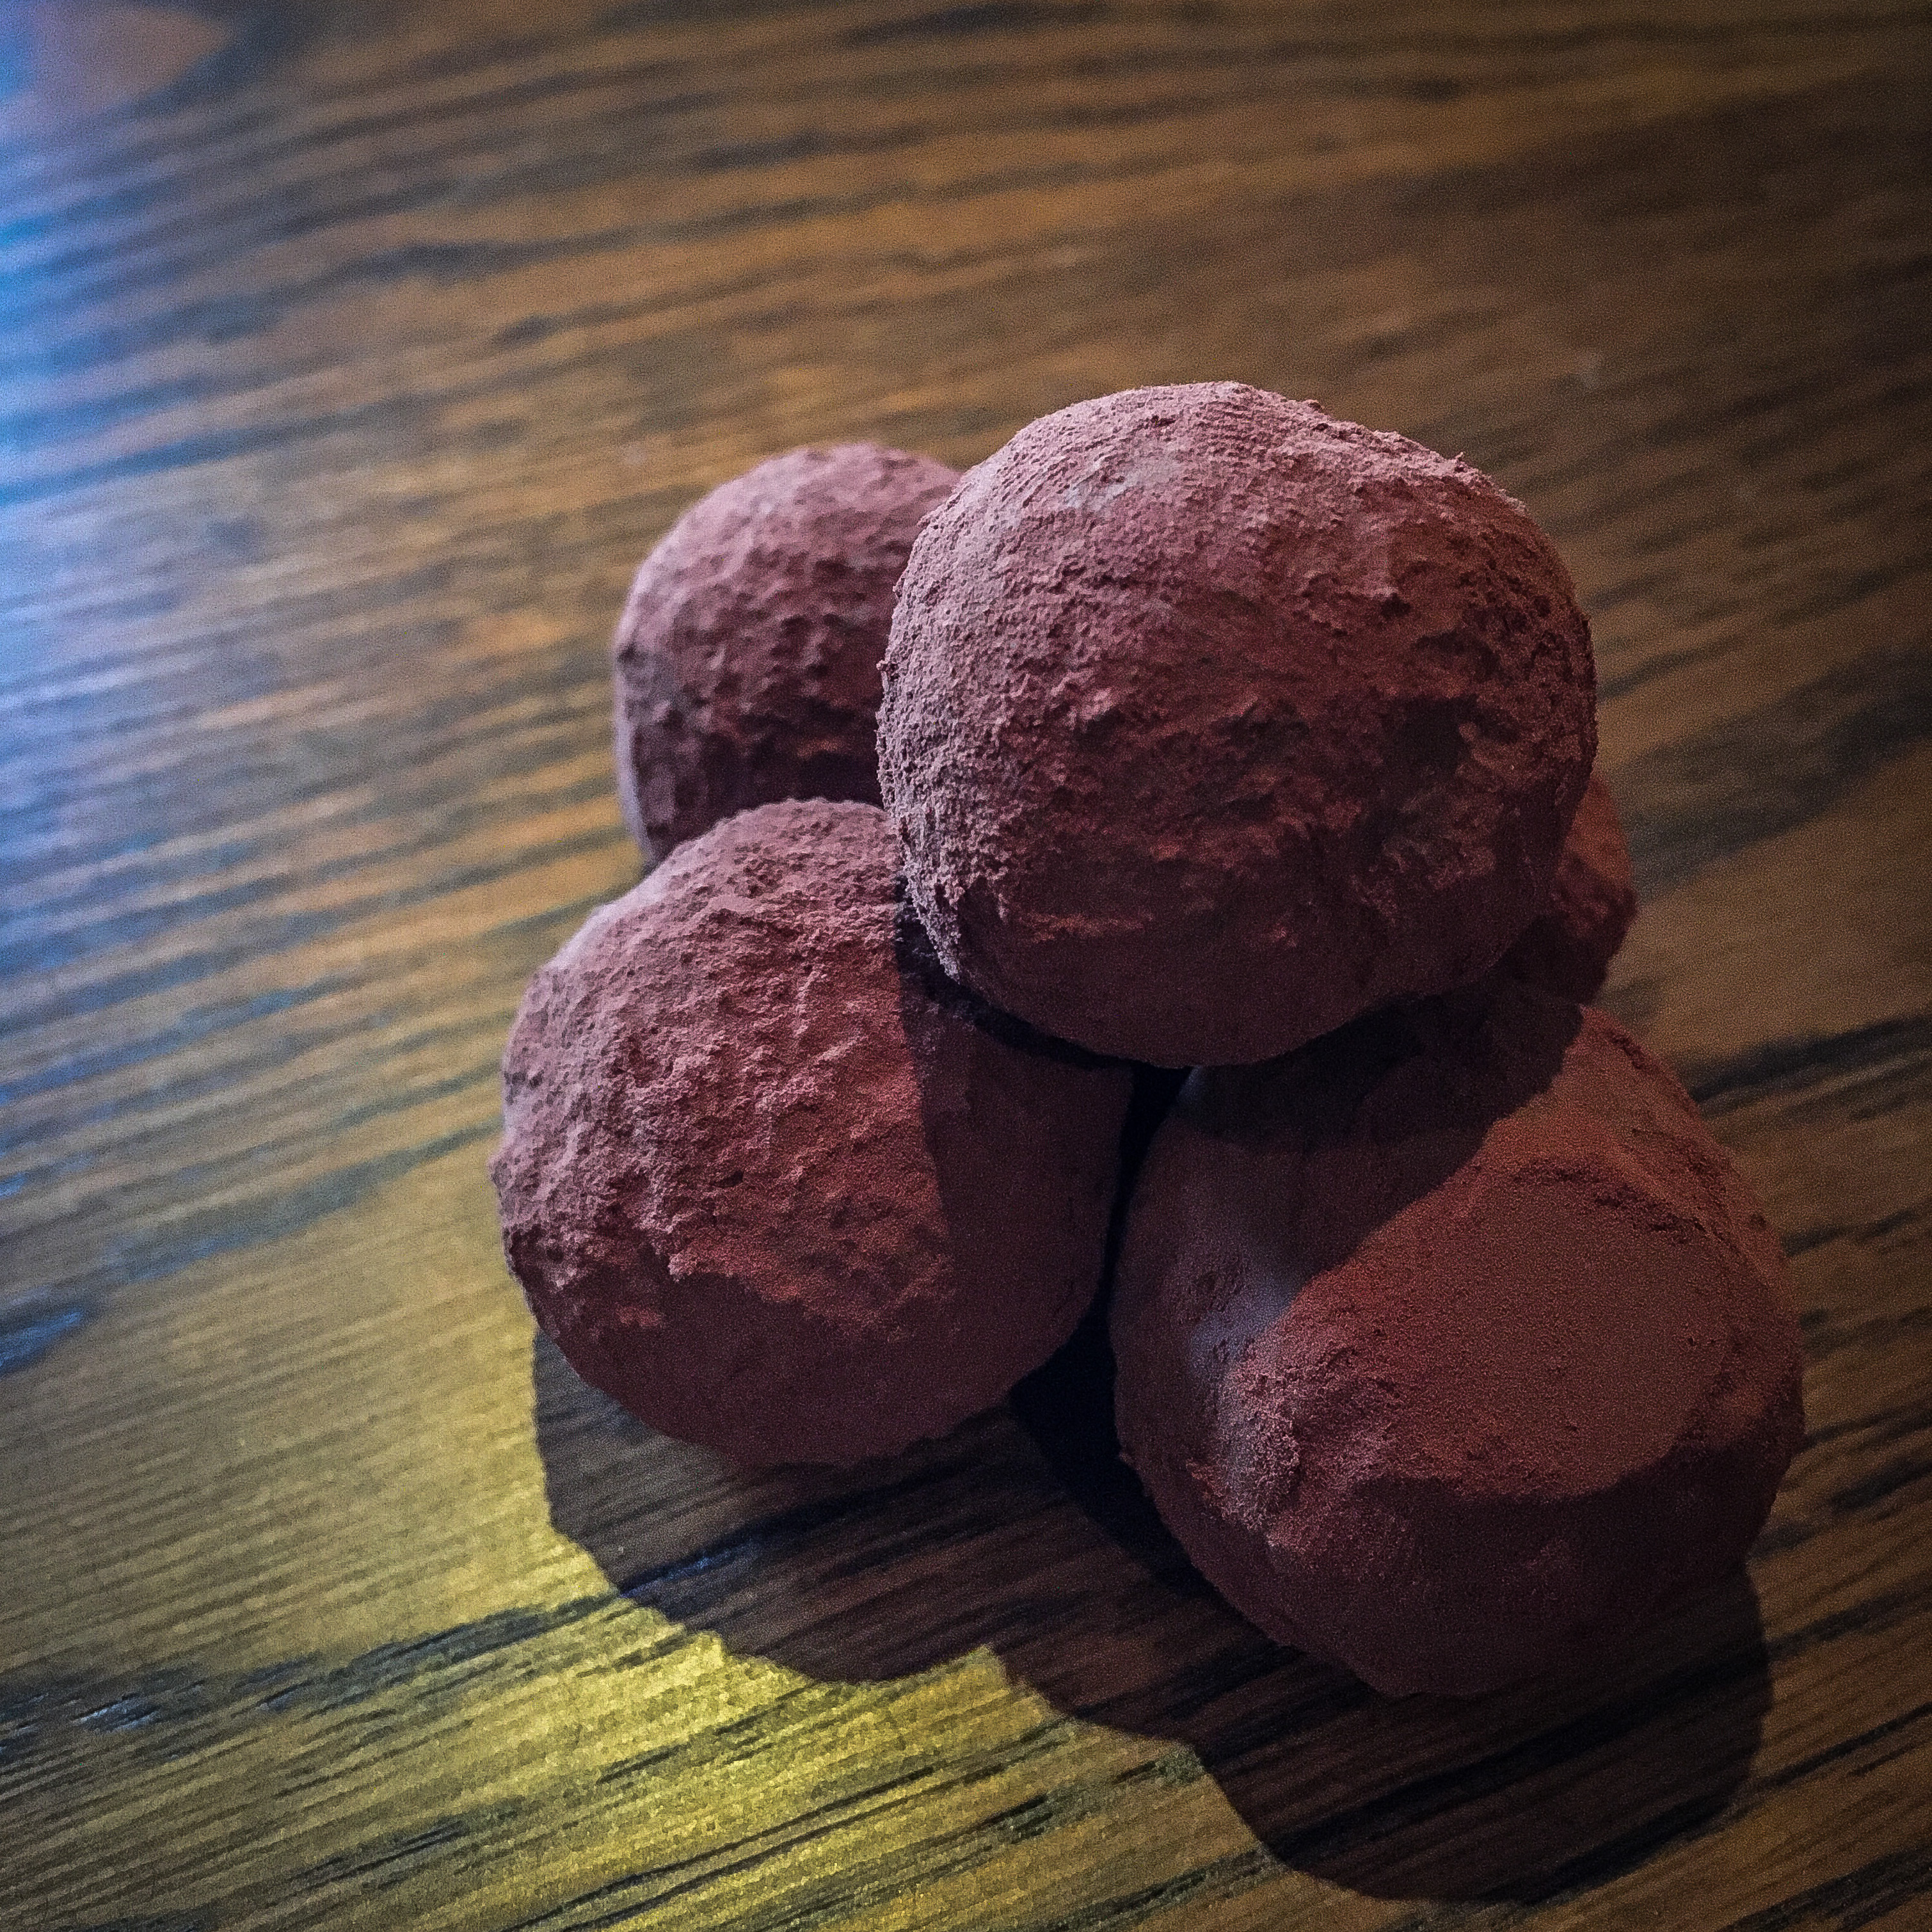
\includegraphics[width=4.25cm,height=7.5cm]{4.png} & 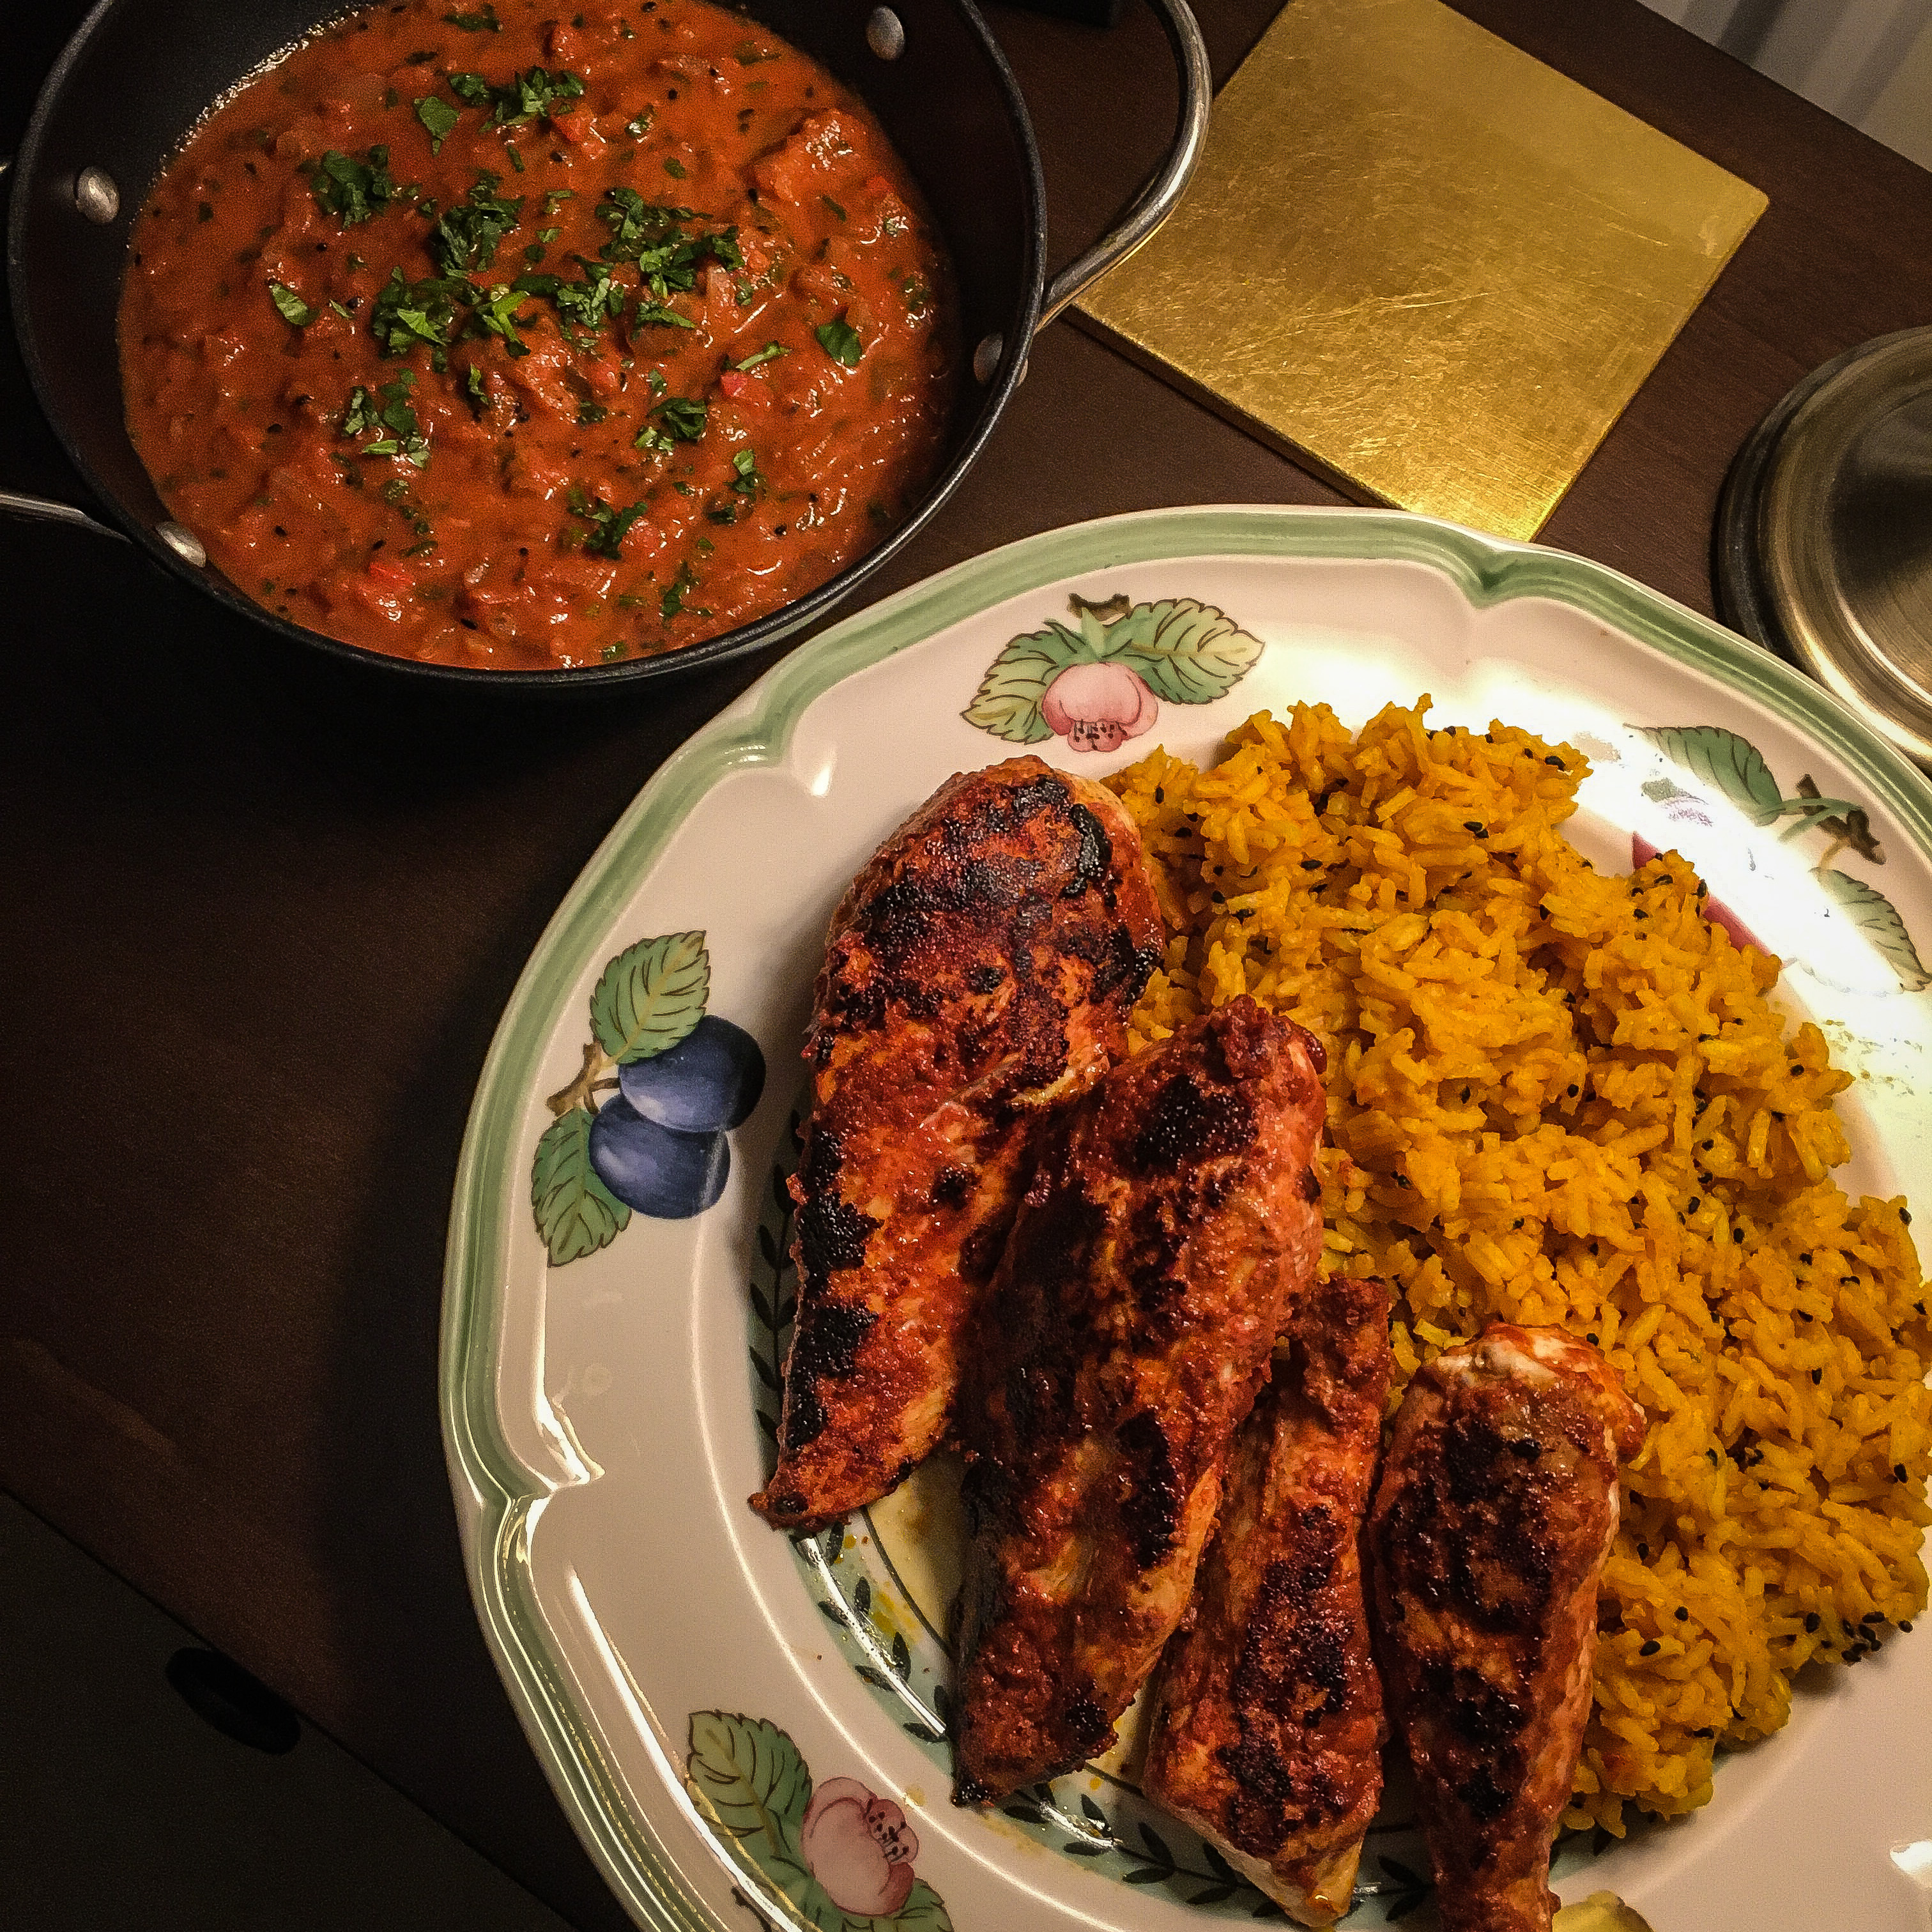
\includegraphics[width=4.25cm,height=7.5cm]{5.png} & 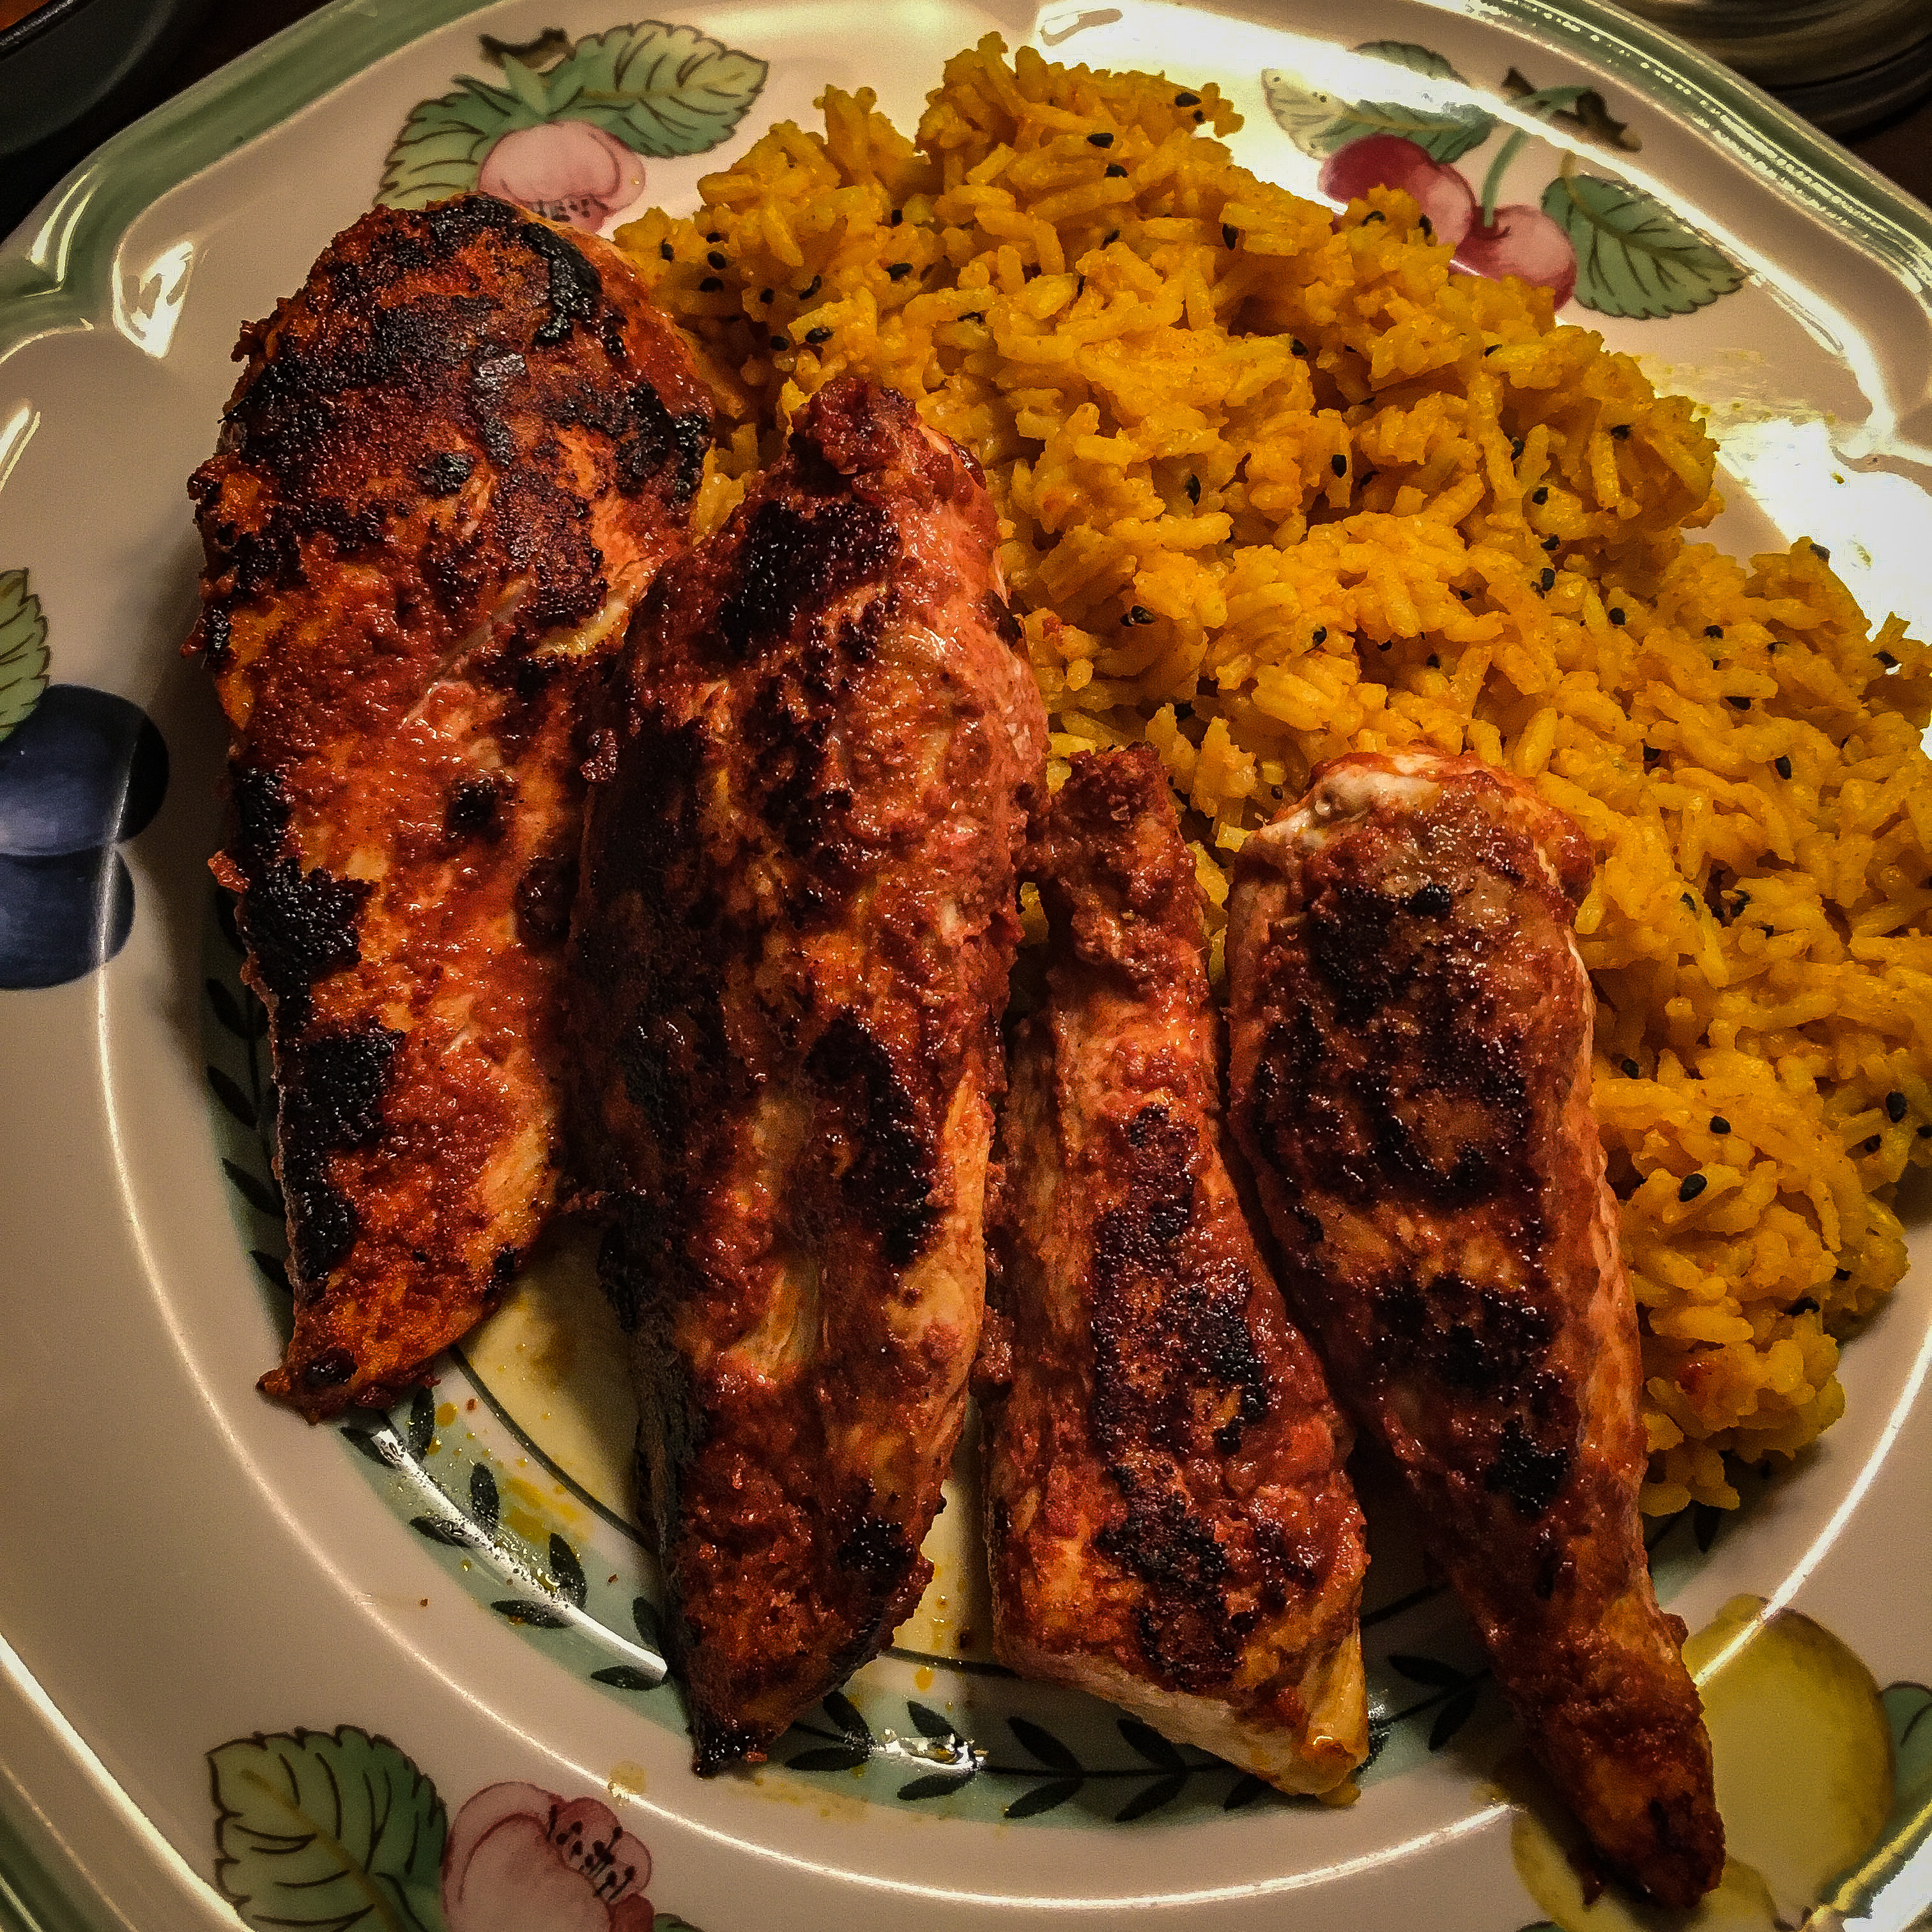
\includegraphics[width=4.25cm,height=7.5cm]{6.png}\\
	\end{tabular}
		\caption{Basic Prototype To-Date}
	\end{center}
	\end{table}

\newpage

\section{Construction}
	
	The primary goal of the construction of this system is to ensure that [1] all functional and non-functional requirements determined by and for clients and users of the final piece are satisfied; and that [2] all components used to construct the system work in harmony and deliver results as efficiently as possible. Briefly with reference to the latter, this is also partially why the HTML-CSS-JavaScript trio was favoured; there is plenty of room for integration of APIs, database back-ends and support for other inclusions extending to JSON use and other styling methods and scripts. They are also universally used respected and can be accessed extremely easily for prototyping and testing purposes, etc With reference to the first element, recall the basic requirements of this system:

	\begin{enumerate}
	\setlength\itemsep{0cm}
		\item Log-in using a username and password (no bloated authentication)
		\item View, edit and request deletion of their account details such as name, residence, gender, height, weight and profile picture
		\item View an overview of their statistics and recent activities
		\item View their personal inputs such as `abilities' and `equipment'
		\item View a weather breakdown using real weather data (OpenWeather API)
		\item View their `rewards'
		\item View their ongoing `challenges and competitions'
		\item Produce results based on user inputs such as their abilities, equipment, rewards and competitions
		\item Access the user's location (Geolocation API)
		\item View an OS map (OS API)
		\item Use and create results from the user's location (OS API, OpenWeather API)
		\item View and create GPS routes
		\item Upload GPX files
		\item Choose a `priority sport' which will be displayed with priority in their overview section
		\item View their current location (latitude/longitude or grid co-ordinates) as two numbers upon request
		\item Use their grid coordinates to quick-request a `random' route suggestion
		\item Display various grid location markers on an OS map
		\item Display various routes on an OS map
		\item Display various guides based upon elements of the system
		\item Offer an appropriate and relevant user interface 
		\item Contain the appropriate accessibility standards
		\item Be ensured that their data is secure and accessible only for the correct purposes
	\end{enumerate}

	The log-in requirement is satisfied in a fairly conventional way; with a log-in system. For prototyping purposes, the system uses basic JSON connectivity with JavaScript to read and write usernames and passwords. As previously mentioned, the usability of this system is very versatile so there isn't much need for extensive scope on the log-in end of things. That is, everyone logging-in to this system will be there for a fairly similar purpose; to engage with their sport activities. Therefore, there is just one log-in option. To create an account, all that is required is an e-mail address, a username and a password. Based people will tell you that the `woke' modern-day 69-factor authentication methods are inane. This is true. Reliance is put on users to ensure they create secure authentication combinations. If this system were ever to be developed further, a more secure data-management back-end with reliable encryption would be implemented.\\

	Once logged-in to their account, as expected, users will be presented with the standard profile details element which displays all of the user attributes which are assigned during the create account process or which have been added at a later date. There is also JavaScript functionality which allows the user to interact with these attributes in order to edit or remove them. Likewise, there is similar element with functionality which displays [1] the aggregate statistics of all activities which a user has partaken in and [2], a summary of the statistics relevant to recent activities determined by the user. Furthermore, the requirements relating to user ability, equipment, weather, challenges and competitions all follow the same format with their respective elements displayed to the user, with intermediary JavaScript computations managing user inputs and final output.

	\subsection{Application Programming Interfaces (APIs)}

	To-date, this system uses three APIs; GPS, weather data, and mapping: Geolocation, OpenWeather and Ordnance Survey, respectively. With further reference to the requirements list, more specifically, the weather requirement makes use of two of these APIs, Geolocation and OpenWeather. The OpenWeather API is used in conjunction with some homemade JavaScript and HTML output which displays live and accurate weather from JSON files hosted by Open Weather, which are update hourly. This is extremely extensible and has actually taken most of my time on this project over the last week as I want the forecasting to be as comprehensive and relevant to the activities on this system as possible. To enhance this feature, the Geolocation API is also integrated to allow users to quickly display the forecast for their current location. This is especially relevant when the users are in the field and once on the site, checking their local weather is just a four-button job. Users can also use Geolocation in an isolated context to simply view their latitude and longitude. At a later date, this will also be translated to the OS grid coordinates.\\

	Furthermore, the Ordnance Survey API is utilized in the `Conquest Map' and `Cruiser Map' portions of the hiking and cycling elements of the system. To-date, this only contains the functionality of displaying the OS 1:250,000 and 1:500,000 Leisure (topographical) maps and therefore only satisfies the `view an OS map requirement'. However in time to come, this will be the most extensible and expansive element(s) of the site; as it will include the abilities to put-to-use the user's location, using Geolocation, to generate route suggestions and display current location, etc.; and, it will use GPX and JSON data to integrate relevant markers and waypoint on the map which users can interact with. The final, `guide', requirement is satisfied in various `keys' and `suggested reading's which appear in their relevant locations throughout the site.

	\subsection{Development Environment}

	The table below summarized all of the languages which are used in the construction of this system, their relationship to the integration of APIs, and the environment in which production is conducted.

	\begin{table}[h]
		\scriptsize
		\renewcommand{\arraystretch}{1.25}
	\begin{center}
	\begin{tabular}{llll}
		\textsc{Purpose} & \textsc{Language} & \textsc{APIs} & \textsc{Environment}\\
		\hline
		UI Functionality & HTML & Geolocation & Command Line $\rightarrow$ Vim $\rightarrow$ .html\\
		& & OpenWeather\\
		& & Ordnance Survey\\
		UI Functionality & JavaScript & Geolocation & Command Line $\rightarrow$ Vim $\rightarrow$ .js, .json\\
		& & OpenWeather\\
		& & Ordnance Survey\\
		UI Functionality & PHP & & Command Line $\rightarrow$ Vim $\rightarrow$ .php\\
		UI Graphic Design & CSS & & Command Line $\rightarrow$ Vim $\rightarrow$ .css\\
		Rear-End Functionality & SQL & & Command Line $\rightarrow$ Vim $\rightarrow$ .sql, .csv\\
		Rear-End Functionality & Python & & Command Line $\rightarrow$ Vim $\rightarrow$ .py\\
		\hline
	\end{tabular}
		\caption{Language Use}
	\end{center}
	\end{table}

	Before going any further, it must be noted that there is and will be NO use of proprietary software throughout this system development. Proprietary software is unreliable, unnecessary, expensive and majorly bloated. Using free and open source software such as the APIs I've chosen, and my selected development environment significantly increases the freedom and extensibility of this project. On the subject, for the last time, my development environment is using the text editor Vim alongside SC-IM comma-separated environment and Brave Browser to create and view the system. This takes place on my Suckless DWM setup on Artix Linux. Zero bloatware. Everything is plain text.\\

	So forth, HTML is used to create the base upon which the system is laid; giving the basic connectivity to the Geolocation, OpenWeather and Ordnance Survey APIs. The use of HTML also allows incredibly easy integration of other features such as scripts which allows intra-HTML typesetting using \TeX\ syntax which makes tasks such as displaying formul\ae\ in the suggested ready far easier. The Font Awesome library is also integrated using HTML to display various universal symbols. This requires a link to a style sheet and often scripts to access additional features.\\

	JavaScript is used to tie-in the functionality of Geolocation, OpenWeather and Ordnance Survey as without the relevant scripts, they would not function. Of course, the inputs and outputs to these APIs can also be altered in various ways by creating custom scripts which interface with them. This has and will be done extensively to make the APIs more relevant to this scenario. Additionally, there are smaller JavaScript elements implemented throughout the system which exist simply to make the usability a little more smooth for the user user. Things such as drop-downs, hiding content, interactive elements, etc.\\

	Alongside JavaScript are various JSON files which are used to store semi-rear-end data and be accessed upon requests such as finding the coordinates of a specific mountain, for example. Or, accessing a user's details upon a log-in request. This is once again fine as the system currently does not have to be secure. CSV files will also be references in the future for other non-functional, context-based data requests. At a later date in development, PHP, SQL and Python will be used to manage, access and manipulate larger-scale back-end storage and requests.\\

	CSS is obviously present to make the site look a little more approachable. Don't think there's much more to be said there. It isn't really required but I'm just about the only person in this institution who thinks a style-free site is better looking than a styled one these days so hey ho. CSS is however, a crucial component in making this system go from just a website to a web application. Using HTML5's CSS integration, the site can fully scale to mobile devices with all of the JavaScript functionality still in tact.

	\subsection{Functionality \& Interaction}

	As this system is a web application, it is based on a series of HTML forms and inputs such as buttons, clicks, text inputs, integer inputs, date inputs, etc., with an HTML-rendered JavaScript semi-back-end. This is how communications are made with the back-end and then produced into raw HTML output form JavaScript computations. Some examples of this interactivity are highlighted in the table below.

\newpage

	\begin{center}
		\scriptsize
	\begin{longtable}{p{3cm}lp{6cm}}
		\textsc{Element} & \textsc{Function} & \textsc{Functionality}\\
		\hline
		\hline
		\multicolumn{3}{c}{\textsc{Page Select (From Any Page)}}\\
		\hline
		\hline
		Link & Go to `Drafting' & Leave current page and go to the `Drafting Room', otherwise known as the home page (index)\\
		Link & Show Hiking elements & Hover over `Hiking' on desktop to show the drop-down list of pages or, click on link embedded in `Hiking' on mobile to show the list\\
		Link & Go to `Conquest Map' & Leave current page and go to the OS map associated with hiking\\
		Link & Go to `Ranger Graphs' & Leave current page and go to the statistics and graphing page associated with hiking\\
		Link & Go to `GPS Route Suggester' & Leave current page and go to the GPS page associated with hiking\\
		Link & Go to `Comprehensive Key' & Leave current page and go to the key of syntax and symbols associated with hiking maps and literature\\
		Link & Go to `Cruiser Map' & Leave current page and go to the OS map associated with cycling\\
		Link & Go to `Ranger Graphs' & Leave current page and go to the statistics and graphing page associated with cycling\\
		Link & Go to `GPS Route Suggester' & Leave current page and go to the GPS page associated with cycling\\
		Link & Go to `Comprehensive Key' & Leave current page and go to the key of syntax and symbols associated with cycling maps and literature\\
		\hline
		\hline
		\multicolumn{3}{c}{\textsc{Drafting Room}}\\
		\hline
		\hline
		\multicolumn{3}{c}{\textsc{Drafting Room: Site Intro/Summary}}\\
		\hline
		Button Function & Request current coordinates & Using an HTML button element, execute a function which uses Geolocation to request the user's current latitude and longitude and display this inner HTML using a JavaScript script\\
		Button Function & Request `nearest project' & Using an HTML button element, execute a function which uses Geolocation (for the user's current coordinates) and compares this to the coordinates of their nearest unconquered mountain, etc. or whatever they're into, and display this inner HTML using a JavaScript script. Obviously this requires a few more variables which are implemented in other areas\\
		\hline
		\multicolumn{3}{c}{\textsc{Drafting Room: Profile}}\\
		\hline
		Link & Go to `Overview' & Hide current profile element and show the statistics overview element using CSS and JavaScript\\
		Link & Go to `Conditioning' & Hide current profile element and show the conditioning element which contains the user attributes such as abilities, equipment and their weather forecast, using CSS and JavaScript\\
		Link & Go to `Rewards' & Hide current profile element and show the rewards element which highlights the pre-determined achievements which the user has gained in the field\\
		Link & Go to `Competitions' & Hide current profile element and show the competitions element which contains a ranking and comparison between the user and other users on mutually conquered field routes\\
		\hline
		\multicolumn{3}{c}{\textsc{Drafting Room: Profile -- Conditioning}}\\
		\hline
		Link & Show `Ability' & Recursively show and hide the element container of attributes associated with the user's ability using CSS and JavaScript. The link for this element is embedded within an external Font Awesome symbol\\
		Link & Show `Equipment' & Recursively show and hide the element container of attributes associated with the user's equipment using CSS and JavaScript. The link for this element is embedded within an external Font Awesome symbol\\
		Link & Show `Wether' & Recursively show and hide the element container of attributes associated with the user's weather forecasting using CSS and JavaScript. The link for this element is embedded within an external Font Awesome symbol\\
		\hline
		\multicolumn{3}{c}{\textsc{Drafting Room: Profile -- Conditioning -- Weather}}\\
		\hline
		Drop-down select & Select a Munro for weather analysis & Using an HTML select element, list pre-determined items (Munros) which have been assigned attributes such as the, relevant here, latitude and longitude, in a JSON file and enter these respectively into the below input fields\\
		Drop-down select & Select a Corbett for weather analysis & Using an HTML select element, list pre-determined items (Corbetts) which have been assigned attributes such as the, relevant here, latitude and longitude, in a JSON file and enter these respectively into the below input fields\\
		Number Input & Enter latitude & Relay manually inputted numbers\\
		Number Input & Enter longitude & Relay manually inputted numbers\\
		Button Function & Request current coordinates & Using an HTML button element, execute a function which uses Geolocation to request the user's current latitude and longitude and enter these respectively into the above input fields\\
		Button Submit & Request weather forecast & Using an HTML button element, execute a function which uses the latitude and longitude inputs to request weather data for that location, using the OpenWeather API, and display this inner HTML using a JavaScript script\\
		\hline
		\caption{System Functionality}
	\end{longtable}
	\end{center}

\newpage

\section{Testing}

	I am a big believer in the ``you don't have to test if you don't make mistakes'' philosophy. Being the command line interfacer that I am, this is usually what I practice. I mean, if you write a shell script and it doesn't work, you'll know about it. So just keep perfecting it until it does exactly what you want it to do. This is after-all, how you learn. It's a similar case with HTML, CSS and JavaScript; especially the first two. You aren't going to know if you've made mistakes, there's nothing to compile so you aren't going to physically see any errors apart from lacking or incorrect content on-screen. This is why using these languages is a far more functional tool in allowing you to learn, develop and produce exactly what it is that you want. Not some inane version of your ideal which a compiler has dictated you into making.

	\subsection{`Test-Driven' Development}

	All of that being said, when developing a web application using HTML, CSS and JavaScript, the developer naturally takes quite a `testy' approach. Just like when you're typesetting a document using Donald E. Knuth's \TeX\ and you compile your document perhaps after every paragraph, new line, table element, figure, etc., to ensure that the formatting is as desired; HTML development adheres to a similar protocol. That is, you are constantly adding very small elements, saving and refreshing your pages in-browser to check your code's integrity; simulating a compilation to some degree. Therefore, technically you are constantly `testing' your code but very minor-to-no errors appear as you make updates in such little increments. And, usually the updates you make are very isolated so will not effect large portions of your code in other locations.\\

	This process also makes the implementation of JavaScript very smooth. For example, you can develop very small elements of JavaScript at a time and call functions, etc., only in very specific locations meaning little portions of HTML input, JavaScript computations and HTML output can be tested in a isolated environment at one time; having minimal effect on the aggregate system. Unless of course, you're one of those Zoomers who puts all of their JavaScirpt in one or two files. That's begging for failure. Anyway, the point is that due to continuous, small-scale testing, there is little room for error and much room to apply these small developments into a much larger context over the entire system once they have been perfected. This process ensures that there is little-to-no opportunity for `technical debt' to accumulate resulting in a backlog of errors and the delay of the development cycle.

	\subsection{Unit Testing Aversion}

	There are actually many tools available to perform unit tests upon browser-relevant JavaScript. These exist for developers to `test the integrity' of JavaScript elements using their relevant HTML counterparts and interfaces. Popular tools such as Unit.js and Mocha are present within development frameworks such as Node.js and in browsers such as Chromium. As you'll be aware of by now, here we are anti-bloatware and anti-spyware and therefore have not and will not be touching any such piece of proprietary software and `big-tech'/government spyware. But that's besides the point anyway. All these tools are deigned to do is allow the developer to write `test cases' which simulate an interfacing instance with the HTML/JavaScript elements. Great, you get an autistic table of results and numerical indicators to five-hundred significant figures which mean little-to-nothing. Maybe on some larger project where results like this need to be scalable and open to more precise analysis, this is relevant. But here, it's simply a waste of time. The method I discussed above which accounts for actual human interaction with the HTML and JavaScript elements on a more continuous basis is not only easier and faster, it lets the developer view their developments with a finer lens and indicates possible enhancements which may not have occurred to them otherwise. 

	\subsection{System Testing}

	This process is usually executed using a team of experts with a clear structural idea of the tree of events in a system and the syntax required to achieve optimal results. Here, there is actually some degree of system testing. The methods relevant in this context are essentially put in place to test whether the functional and non-functional requirements determined previously are met. That is, how the system flows as a whole and how the different HTML and JavaScript elements align to produce a path from one requirement to the next. Further, how CSS has been implemented to satisfy more specific, perhaps industry or context-relevant, requirements. Of course, this process is still a while away from actually being relevant so there isn't a great deal to report apart from that. The process could actually take place using a small dedicated group testers, given their compliance. And like of me.

	\subsection{User Acceptance (UAT), Accessibility \& Usability}

	As the preliminary stages of development are focuses more so on the functionality of the user interface and its interaction with the semi-back-end, there isn't, to-date, much need for accessibility and usability testing. For example, it doesn't matter yet if users cant see the page header properly. As long as I can see it, I can develop upon it. However, as time goes on, it is especially important to ensure that interactive elements, which will be open for constant interface with the users, are easily usable for the varying scope of the masses and integral. This is obviously highly relevant to various aspects of the user interface . The testing process here will likely consist of regular but small surveys based on small samples of the system which will question users on their interactive experience. Given this regular feedback, it should be easy to keep all elements in harmonious continuity. Using a fair scale and scope of individuals in the sample will provide accurate aggregate quantitative and qualitative results. It's likely this element of development will be outsourced to a larger group of less-development-experienced/realistic individuals.\\
	
	User Acceptance Testing is a critical stage in determining the integrity and usability of the final system. It takes into account many of the elements present in the system testing protocol, in that it is the final stage of testing and the flow of the entire system should be seamless at this point. Like most of this testing section, this is still far from tangibility. However, it is important when developing each individual component of the system to keep in mind the overall structure of the system and how an element may be relevant to another. This is key step in ensuring consistency and coherence with the brief of requirements. When the time comes to hand over the system to dedicated testers, a clear recursive tree of events will be mapped which allows a comprehensive overview of what should and shouldn't be present and therefore, function. It's likely that this step will be executed by myself and one or two other experienced individuals in the field.
	
\end{document}
